\section{Theorie}

\subsection{Zielsetzung}

Mithilfe des Geiger-Müller-Zählrohrs kann in der Kernphysik die Intensität von
ionisierter Strahlung gemessen werden. Der folgende Versuch behandelt
die Funktionsweise eines Geiger-Müller-Zählrohrs und seine Charakterisierung
über verschiedene Messungen, um die Kenndaten des vorliegenden Gerätes zu ermitteln.

\subsection{Aufbau und Wirkungsweise}

Das Geiger-Müller-Zählrohr besteht im Wesentlichen aus einem Kathodenzylinder
mit einerm axial verlaufenden Anodendraht (siehe Abb. \ref{fig:Geiger}). Um die
später genauer beschriebenen Nachentladungseffekte gering zu halten, ist das
Zählrohr zusätzlich mit einem alkoholhaltigem Gasgemisch gefüllt. Wird eine
äußere Spannung angelegt, so entsteht zwischen Kathode und Anode ein
radialsymmetrisches elektrisches Feld. Dringt nun ein Teilchen in das Zählrohrvolumen ein,
so werden abhängig von der angelegten Spannung nach der Primäriosation
verschiedene Effekte hervorgerufen (siehe Abb. \ref{fig:Bereiche}).

\begin{figure}
  \centering
  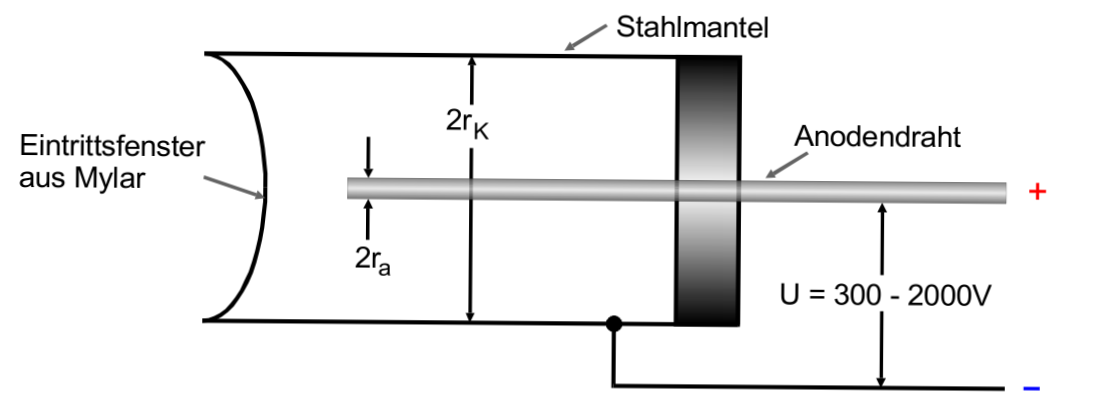
\includegraphics[width=\textwidth]{Zaehlrohr.png}
  \caption{Aufbau des Geiger-Müller-Zählrohrs. \cite{anleitung01}}
  \label{fig:Geiger}
\end{figure}

Bei einer geringen Spannung gelangen durch Rekombination bedingt nur sehr
wenige Elektronen an die Anode (Bereich I, Abb. \ref{fig:Bereiche}). Wird die
angelegte Spannung weiter erhöht, gelangen aufgrund der höheren Feldstärke nahezu
alle Elektronen an die Anode und die Rekombinationswahrscheinlichkeit nimmt
stark ab. Geräte die in diesem Spannungsbereich eingesetzt werden, werden als
Ionisationskammern bezeichnet (Bereich II, Abb. \ref{fig:Bereiche}).
In dem bezeichneten Bereich ist der Ionisationsstrom proportional zu Energie bzw.
Intensität der einfallenden Strahlung.

Wird die Feldstärke weiter erhöht können die freigesetzten Elektronen
genügend Energie aufnehmen um ihrerseits ionisieren zu können. Bei einer hinreichend
hohen angelegten Spannung wird durch die Stoßionisation die Zahl der freigesetzten
Elektronen stark erhöht, dieser Vorgang wird als Townsend-Lawine bezeichnet.
Die gesammelte Ladung Q ist aber immer noch proportional zur Primärteilchenenergie,
weshalb in diesem Bereich arbeitende Detektoren auch als Propotionalitätszählrohr
bezeichnet werden (Bereich III, Abb. \ref{fig:Bereiche}).

Bei einer erneuten Erhöhung der Betriebsspannung gelangt man in den Auslösebereich,
welcher den eigentlichen Arbeitsbereich des Geiger-Müller-Zählrohrs klassifiziert
(Bereich IV, Abb. \ref{fig:Bereiche}).
Hier breitet sich die Entladung aufgrund von vielzahlig
freigesetzten UV-Photonen im gesamten Zählrohrvolumen aus. Die gesammelte Ladung
ist nun nicht mehr von der Primärionisation abhängig, sondern nur noch von
dem Zählrohrvolumen und der angelegten Betriebsspannung.

Der sich an den Auslösebereichs anschließende Bereich wird als Entladungsbereich
bezeichnet (Bereich V, Abb. \ref{fig:Bereiche}. Die Nachentladungen sind
in diesem Bereich so groß, das von einer eigenständigen Gasentladunge gesprochen wird.
Ein einzelnes ionisierendes Teilchen kann eine Dauerentladung hervorrufen.
Das Messgerät wird in diesem Bereich schnell zerstört, weshalb die Betribsspannung
diesen Bereich nicht erreichen sollte.

\begin{figure}
  \centering
  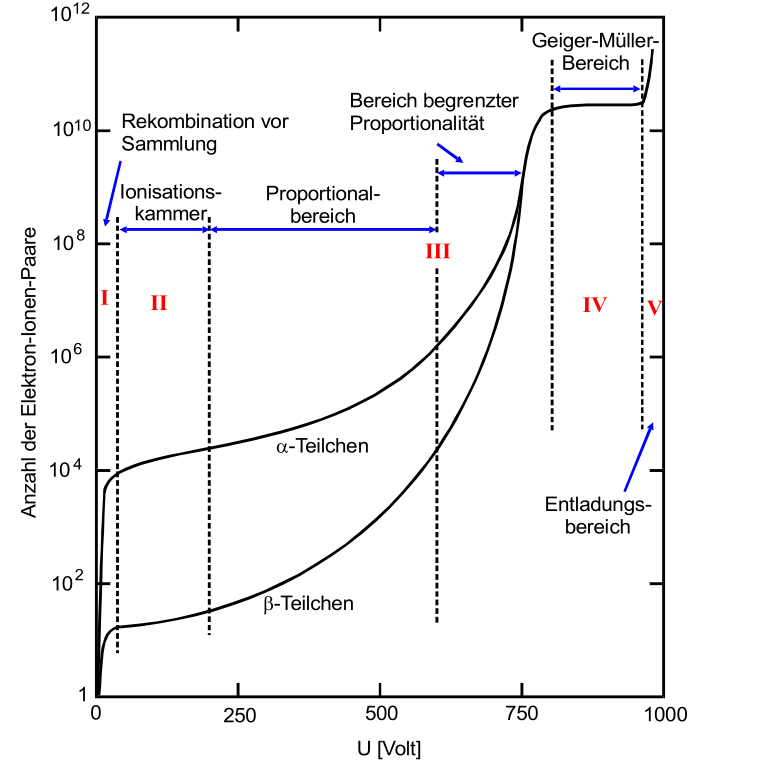
\includegraphics[width=\textwidth]{Bereiche.png}
  \caption{Die verschiedenen Bereiche im Bezug auf die angelegte Betriebsspannung.\cite{anleitung01}}
  \label{fig:Bereiche}
\end{figure}

\newpage

\subsection{Einfluss der positiven Ionen}

Die freigesetzten positiven Ionen bauen mit der Zeit im Zählrohr eine positive
Raumladung auf, welche einige Störeffekte hervorruft. Einerseits wird die
Feldstärke zwischenzeitlich so stark gesenkt, dass eintreffende Teilchen vom
Zählrohr nicht mehr registriert werden. Diesen Zeitraum nennt man auch Totzeit $\Tau$.

Nach Auflösen bzw. Abwandern der positiven Raumladung wird stufenweise wieder eine
Lawinenbildung möglich, bis nach vollständiger Neutralisierung der Ionen nach der
Erhohlungszeit $t_{\symup{Erholung}}$ wieder Ladungsimpulse in ihrer ursprünglichen Höhe erreicht
werden.

Ein weiterer Störeffekt sind die Nachentladungen. Diese entstehen wenn im Zählrohrmantel
auftreffende Ionen Elektronen aus der Metalloberfläche freisetzen, wodurch mehrere
zeitlich versetzte Ausgangsimpulse erzeugt werden. Dieser Effekt ist höchst unerwünscht,
da er das Auftreffen von ionisierten Teilchen vortäuscht. Er kann aber durch die anfangs
erwähnten Alkoholdämpfe im Zählrohr reduziert werden. Die frei werdende Energie
bei Stößen führt hier nicht zur Emission eines Elektrons sonder regt lediglich
die Schwingung eines vielatomigen Alkoholmoleküls an. Die Nachentladungen
können nicht vollständig verhindert werden, sondern werden ledinglich reduziert.

\subsection{Charakteristik des Zählrohrs}

Die Charakteristik eines Zählrohrs erhält man, wenn die registrierte Teilchenzahl
N gegen die angelegte Spannung bei konstanter Strahlungsintensität aufgetragen wird.

\begin{figure}
  \centering
  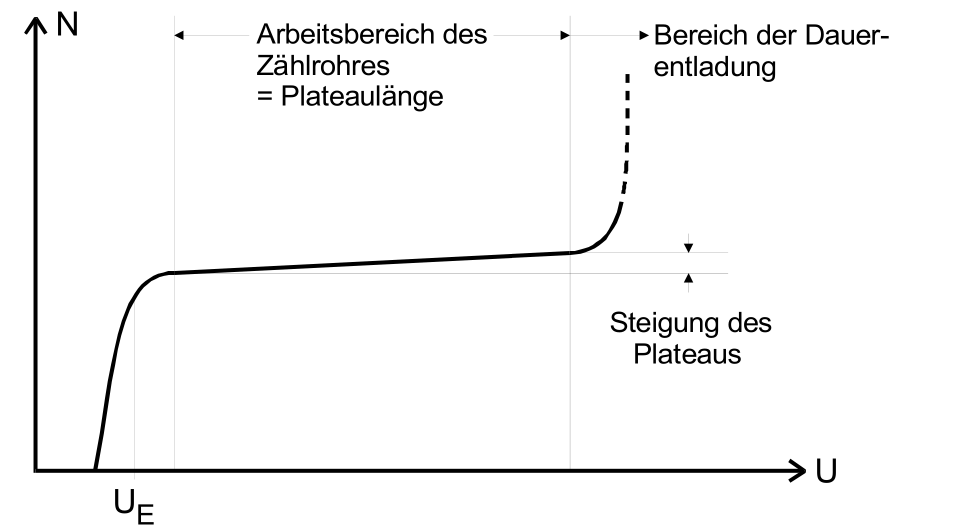
\includegraphics[width=\textwidth]{Charakteristik.png}
  \caption{Zählrohrcharakteristik bei konstanter Strahlungsintensität. \cite{anleitung01}}
  \label{fig:Charakteristik}
\end{figure}

Der lineare Teil der in Abb. \ref{fig:Charakteristik} zu sehenden Kurve heißt
Plateau. Durch Betrachtung der Plateausteigung sowie Spannungsmäßigen Ausdehnung
lässt sich eine Aussage über die Qualität des verwendeten Zählrohrs treffen, da
im Idealfall die Steigung Null sein sollte und die Ausdehnung möglichst groß.
Aufgrund der Nachentladungen wird jedoch eine geringe Zunahme von N erkennbar sein.
Bei zu hoher Spannung wird die Zahl der Nachentladungen so groß, dass der Entladungsbereich
erreicht wird (Bereich V, Abb. \ref{fig:Bereiche}.

\subsection{Ansprechvermögen des Zählrohrs}

Unter dem Ansprechvermögen wird die Wahrscheinlichkeit, dass ein in den
Detektro einfallendes Teilchen im Zählrohr nachgewiesen wird, verstanden.
Das Ansprechvermögen für geladene Teilchen wie $\alpha$- und $\beta$-Teilchen ist
nahezu bei 100 \%. Jedoch werden sie im metallischen Zählrohrmantel vollständig
absorbiert. Um das Zählrohr dennoch abschließen zu können,
wird bei den Endfensterzählrohren an der Stirnseite eine Mylar-Folie angebracht.
Diese besteht aus Atomen niedriger Ordnungszahl und lässt die Teilchen dennoch passieren.
Selbst $\alpha$-Teilchen werden von der Folie nicht absorbiert und können
diese durchdringen.
Aufgrund des Unterdruckes ist die Folie leicht nach Innen gewölbt (Abb. \ref{fig:Geiger}).

Das Ansprechvermögen von Photonen ist begründet durch ihre fehlende Ladung äußerst
gering, sodass eine Messung mit einem Geiger-Müller-Zählrohr lediglich bei
sehr hoher $\gamma$-Intensität sinnvoll ist.

\newpage

\section{Aufbau und Durchführung}

\begin{figure}
  \centering
  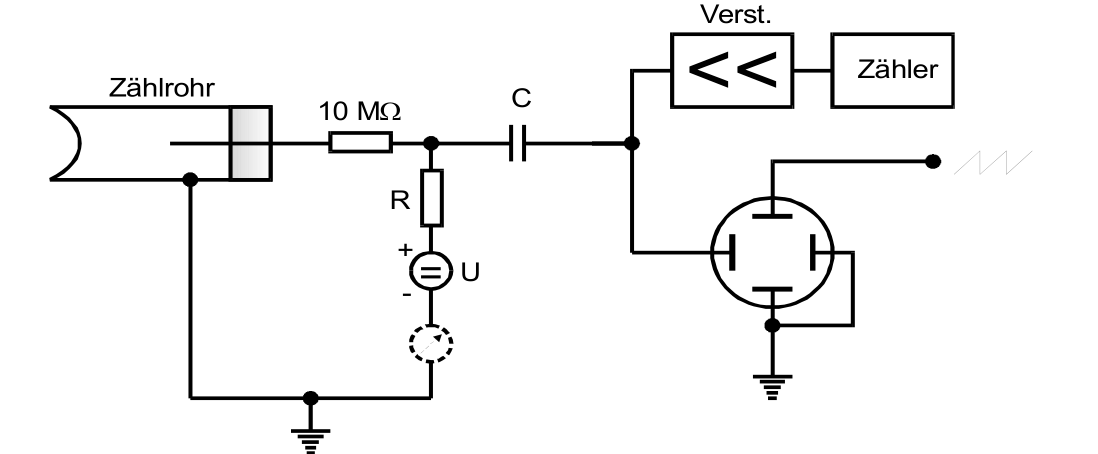
\includegraphics[width=\textwidth]{Aufbau.png}
  \caption{Aufbau der verwendeten Messapparatur. \cite{anleitung01}}
  \label{fig:Aufbau}
\end{figure}

Bei den folgenden Experimenten wird ein Aufbau gemäß Abbildung \ref{fig:Aufbau}
verwendet. Dabei fließt die auf dem Zähldraht gesammelten Ladung Q über
den Widerstand R ab. Der entstehende Spannungsimpuls wird über einen Kondensator
ausgekoppelt, im Verstärker vergrößert und im Zahlgerät registriert oder auf einem
Oszilloskop sichtbar gemacht.

Im ersten Teil des Experimentes wird bei einer Probe die Abhängigkeit von gemessener
Teilchenzahl und Ionisierungstrom von der angelegten Spannung gemessen. Dafür wird
am Anfang eine Spannung von $\num{300}\su{V}$ angelegt, die dann in $\num{10}\su{V}$ Schritten
bis auf $\num{700}\su{V}$ erhöht wird.
Dabei werden nach jedem Schritt der Ionisierungsstrom, sowie die in einem
Zeitintervall von $t = \num{60}\su{s}$ auftreffenden Teilchen notiert.

Im nächsten Teil des Experimentes werden auf dem Oszilloskop die Totzeit und die
Erhohlungszeit bei einer Spannung von $U = \num{450}\su{V}$ ausgemessen. Zudem werden
die Nachentladungen sichtbar gemacht und beobachtet.

Zum Abschluss wurde mit dem Zählrohr noch die eintreffende Teilchenzahl der
Probe $N_1$, der Proben $N_1$ und $N_2$ kombiniert sowie der Probe $N_2$ alleine
bei einer Spannung von $U = \num{450}\su{V}$ gemessen. Auf diese, unter dem Namen
Zwei-Quellen-Methode bekannte Methode wird in der Auswertung verschärft eingegangen.
